\documentclass[conference]{IEEEtran}
\IEEEoverridecommandlockouts

\usepackage{cite}
\usepackage{amsmath,amssymb,amsfonts}
\usepackage{algorithmic}
\usepackage{graphicx}
\usepackage{textcomp}
\usepackage{xcolor}
\def\BibTeX{{\rm B\kern-.05em{\sc i\kern-.025em b}\kern-.08em
    T\kern-.1667em\lower.7ex\hbox{E}\kern-.125emX}}
\begin{document}

\title{DNA Sequence Classification for Detection of Plasmid Fragments}

\author{
\makebox[.25\linewidth] {Mehnaz Yunus} \\
\textit{Department of Computer Science and Engineering} \\
\textit{National Institute of Technology Karnataka}\\
Surathkal, Mangalore, India \\
mehnaz138@gmail.com \\

\and
\makebox[.5\linewidth] {Sharanya Kamath} \\
\textit{Department of Computer Science and Engineering} \\
\textit{National Institute of Technology Karnataka}\\
Surathkal, Mangalore, India \\
16co140.sharanya@nitk.edu.in \\

\and
\makebox[.5\linewidth] {Nagaratna B Chittaragi} \\
\textit{Department of Computer Science and Engineering} \\
\textit{National Institute of Technology Karnataka}\\
Surathkal, Mangalore, India \\

\and
\makebox[.25\linewidth] {Shashidhar G Koolagudi} \\
\textit{Department of Computer Science and Engineering} \\
\textit{National Institute of Technology Karnataka}\\
Surathkal, Mangalore, India \\

}

\maketitle

\begin{abstract}
DNA classification is the problem of identifying the functionality of genes using only the sequence information (ATGTGT...) automatically. To understand the functions of different genes and proteins, sequence classification has attracted a lot of attention in genomic research. Plasmids are circular or linear double-stranded DNA molecules which are capable of autonomous replication and are transferable between different bacteria. Computational methods for prediction of genomic elements such as genes are significantly different for chromosomes and plasmids, hence raising the need for separation of chromosomal from plasmid sequences in a metagenome.

We developed a machine learning model for discrimination between plasmid-derived and chromosome-derived sequences.
\end{abstract}

\begin{IEEEkeywords}
DNA sequence classification, bi-directional lstm, recurrent neural networks, plasmids
\end{IEEEkeywords}

\section{Introduction}
Sequence classification has a broad range of real-world applications. In genomic research, classifying protein sequences into existing categories is used to learn the functions of a new protein. In health-informatics, classifying ECG time series (the time series of heart rates) tells if the data comes from a healthy person or comes from a patient with heart disease. In anomaly detection/intrusion detection, the sequence of a user’s system access activities on Unix is monitored to detect abnormal behaviors. In information retrieval, classifying documents into different topic categories has attracted a lot of attentions. Other interesting examples include classifying query log sequences to distinguish web-robots from human users and classifying transaction sequence data in a bank for the purpose of combating money laundering.
\newline

Generally, a sequence is an ordered list of events. An event
can be represented as a symbolic value, a numerical real value, a vector of real values or a complex data type. In this paper, we consider sequence data to be a DNA sequence composed of four amino acids A, C, G, T and a DNA segment, such as ACCCCCGT sequence. In conventional sequence classification, each sequence is associated with only one class label and the whole sequence
is available to a classifier before the classification.
\newline

Next-generation sequencing technologies generate large amounts of biological sequence information in the form of DNA/RNA sequences. Analysis of DNA sequences is important in preventing the evolution of viruses, bacteria, and also used to diagnose disease during an early stage.

Deep Neural Networks (DNNs) have already been adapted for genomics problems such as motif discovery, predicting the deleteriousness of genetic variants, and gene expression inference.

\section{Literature Survey}
A powerful predictive model for the function of noncoding DNA can have enormous benefit for both basic science and translational research because over 98\% of the human genome is noncoding and 93\% of disease-associated variants lie in these regions.
\newline

Traditionally, analyzing DNA sequences involves searching for common motifs or through phylogenetic comparison against known DNA sequences. As such, classifying a new DNA sequence relies heavily on feature engineering using prior knowledge and experts for annotation. Previous work by Asgari et al. demonstrated that word2vec vectors representing trigrams of amino acids could be trained on large amounts of protein sequence data. The resulting vector representation maintained known biological relationships and were successfully used as features for protein family classification.
\newline

To bridge the growing gap between sequenced and annotated DNAs, many computational methods have been established. A majority of these methods employ machine-learning techniques such as Artificial Neural Networks (ANNs) and Support Vector Machines (SVMs). Other computational methods are based on the
analysis of amino acid propensities, physicochemical properties and statistical potential. Complementary methods can be combined to form meta-predictors, which employ the outputs from other classifiers to form their own enhanced predictions.
\newline

Recently, the application of deep neural networks with more than two hidden layers to proteins has permitted a better learning of deep and complex relationships between sequences, structures and functions of amino acids, and advanced the accuracy of pairwise contact prediction, secondary structure and solvent accessible surface-area prediction and protein disorder prediction. However, common deep learning techniques, such as recurrent neural networks and window-based artificial neural networks, while effective at propagating local errors within sequence neighbors, are ineffective at modeling long-range (non-local) interactions between amino acid residues that are structural but not sequence neighbors. Because residue–residue interactions are dominated by structural neighbors, how to account for them is the key for improving sequence-based prediction of protein structural and functional properties.
\newline

The long-range dependence between a series of time-resolved
events can be better captured by enforcing the constant error flow so that useful long-range interactions can be memorized. In this Long Short-Term Memory (LSTM) network, hidden layers are made of memory blocks containing one or more LSTM cells. Each LSTM cell has the discretion to either forget, input to or output the Constant Error Carousel (CEC, i.e. a fixed weight of 1 in the absence of outside signal). The CEC passes through every LSTM cell in the entire sequential event, acting as a
memory backbone effectively connecting the whole sequence, in either the forwards or backwards directions. LSTM-based neural networks have successfully applied to speech and image-related problems in which long range memory is the key for accurate interpretation and prediction.
\newline

Neural Networks (NNs) models have achieved state-of-the-art performance on language modeling tasks in recent years and are now seeing adoption for biological problems. Analysis of DNA sequences is important in preventing the evolution of viruses, bacteria, and also used to diagnose disease during an early stage.From the existing work, the authors absorb some clustering algorithm and data analytics techniques like K-mean, k-mer, KNN, SVM, random forest correlation coefficient, and eigenvalue vector are used for predicting neurological disease. \newline
Currently implementated methods for plasmid-chromosomal classification:
\begin{itemize}
    \item Support Vector Machine\newline
    The SVM is a machine learning technique with a strong theoretical foundation that has been used to improve classification accuracy in biological applications such as the detection of protein family members. kmer based SVM gave an average classification accuracy of 0.871625.

    \item Random Forest.\newline
    In random forest classification, trees are trained based on random selections of genes and strains, genes with the same occurrence pattern could get different contribution scores. This score is an estimate of how important a gene is to correctly classify a certain strain. Additionally, genes that are either present or absent in (almost) all queried strains have negligible impacts to separate strains of differing phenotypes. Random Forest gave a classification accuracy of 0.791423.
\newline

The aforementioned methods have obviously facilitated the development of this important field. However, further studies are still required. Almost all the machine learning methods require fixed length vectors as inputs. Nevertheless, the lengths of DNA sequences vary significantly. During the vectorization process, the sequence-order information and the position dependency effects are lost, and this information is critical for DNA sequence analysis and nucleic acid analysis. Although some studies attempted to incorporate this information into the predictors, it is never an easy task due to the limited knowledge of DNA sequences.
\end{itemize}

\section{Problem Description}
We attempt to classify DNA sequences into either plasmid or chromosomal, by learning the features present in the DNA character sequence using LSTM networks.
The various tools, procedures, methodologies and algorithms available for DNA classification are to be analysed  and compared to find the best and most effective. 

A suitable dataset for the purpose is to be found and if not found, one is to be created by manually labelling the fetched tweets.

Improvement of performance of prediction to initial implementation of DNA classification is attempted. The accuracy of prediction of chromosomal or plasmid in the considered dataset by using the trained model is to be analysed and further improvisation of the accuracy is to be attempted.


\section{Methodology}   

\subsection{Workflow}
We start with character level prediction on DNA sequences. Here, we test whether an LSTM model can accurately predict the next character in a DNA sequence, for manufactured sequences. This will show whether the chosen model is suitable for the classification task or not.

To confirm that an LASTM can model the structure within a genomic sequence, we first train a simple character-level LSTM to predict one of the four possible characters given the previous string of characters. If the LSTM does not give the accuracy as expected, then we will have to more carefully tweak our model until we can identify some signal. We will also use this simpler task to help choose a proper model architecture. 

Once we have empirical evidence that an LSTM can capture the non-random structure within a genome, we explore a sequence classification problem. The DNA classification task into chromosomal and plasmid is carried out next.

\subsection{Dataset}
In recent years, a large amount of DNA and protein sequences are available in public databases, such as GenBank, EMBL Nucleotide Sequence Database and the Entrez protein database.

The two tasks we performed used different datasets.

For character level genome prediction, our baselines were the artificial genomes. Any model that does not perform as expected on these two genomes will not be used for future experiments.
Two genomes were prepared:
\begin{itemize}
    \item A length-3000 repeating genome where the repeated unit is AGCTTGAGGC.
    \item A length-3000 random genome.
\end{itemize}

For binary classification of DNA sequences the dataset used was from the CAMI project and was obtained from NCBI(National Center for Biotechnology Information) archives. It contained E. Coli complete genomes and plasmids. This dataset contains 3000 DNA sequences of length 500, each with a label indicating whether the sequence is plasmid or chromosomal. 

\subsection{Character Level Prediction}
For the character level prediction, an LSTM model with 75 memory cells was used. If this model does not perform as expected on these two genomes, it would point to LSTMs being unable to properly model DNA behaviour.
\begin{itemize}
    \item Accuracy for repeating genome: 1.0 after 25 epochs
     \item Accuracy for random genome: 0.25 after 25 epochs
(as expected).
\end{itemize}

These experiments showed that an LSTM model may be appropriate for modeling a genomic sequence.

\subsection{Bidirectional LSTM (BLSTM)}
A bi-directional long short-term memory network (BLSTM) is a variant of the RNN that combines the outputs of two RNNs, one processing the sequence from left to right, the other one from right to left. Instead of regular hidden units, the two RNNs contain LSTM blocks, which are smart network units that can remember a value for an arbitrary length of time. BLSTMs can capture long-term dependencies and have been effective for other machine learning applications such as phoneme classification, speech recognition, machine translation and human action recognition. Although BLSTMs are effective for studying sequential data, they have not been applied for DNA sequences.

\begin{figure}[h]
\centering
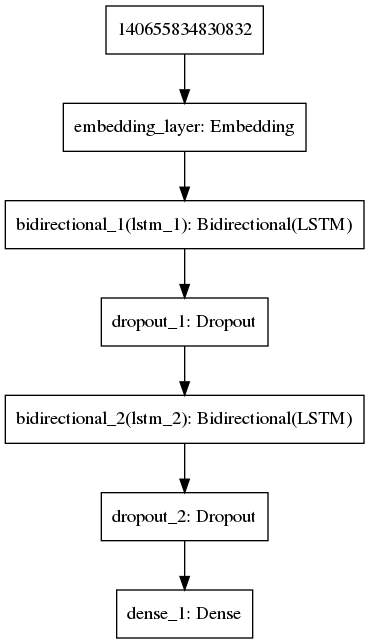
\includegraphics[width=3in]{model.png}
\DeclareGraphicsExtensions.
\caption{Model}
\label{fig_sim}
\end{figure}
% 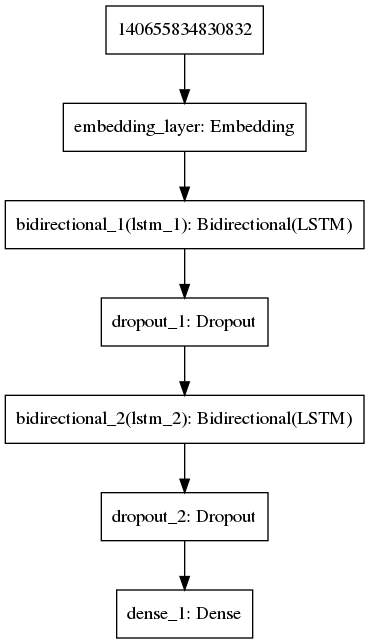
\includegraphics[width=\textwidth]{model.png}

\subsection{Sequence classification}
The  model used contains six layers. The input goes to an embedding layer in which the ACGT sequence is embedded to numerical data. This is followed by 2 sets of bidirectional layer and dropout layer which randomly drops out 20\% of the neurons. Finally there is a fully connected layers which produces the final output.The input layer is designed to encode the pseudo protein by one-hot encoding. Bidirectional LSTM extracts the dependency relationships between subsequences. We take the advantages of every intermediate hidden value from bidirectional LSTM to better handling the long
length of DNA sequences. More comprehensive dependency information can be included into the hidden values by using bidirectional LSTM. Then, those intermediate hidden values are connected to the  dense layer. Because memory cells in one block
extract different levels of dependency information, the  dense layer is designed to weight the dependency relationships extracted from different cells. The outputs of the dense layer are concatenated into one feature vector and be fed into the
output layer for prediction.\newline
With this neural network, both the long and short dependency information of pseudo proteins can be captured by tapping the information from every mediate hidden value of bidirectional LSTM.
\newline

The learning rate was determined in initial training, where larger learning rates of >0.001 did not enable the network to converge. We employed the step learning rate decay technique to reduce the learning rate by 1\% per epoch. That is, the learning rate was initialized at 0.001, and then systematically annealed to 6*10\^-4 within 50 epochs. This allowed the model to
learn finer detail as it progressed through training. Finally, the two outputs of this network are squeezed into a probability distribution through the use of the softmax function.
\newline

\textit{Cross-Validation}\newline
We used 5-fold cross-validation in which the original sample is randomly partitioned into 5 equal sized sub-samples. Of the 5 sub-samples, a single sub-sample is retained as the validation data for testing the model, and the remaining 4 sub-samples are used as training data. The cross-validation process is then repeated 5 times, with each of the 5 sub-samples used exactly once as the validation data. The 5 results are then averaged to produce a single estimation. The advantage of this method over repeated random sub-sampling is that all observations are used for both training and validation, and each observation is used for validation exactly once.

\section{Results and Discussion}
The results of the character level prediction fully match the expected results, giving 1.0 for the repeated sequence and 0.25 for the random sequence. We thus proceeded to the next task.
\newline

For the DNA classification, performance is assessed through the analysis of binary labels and raw prediction values. The raw prediction probabilities are obtained at the output of the network through the use of the softmax function. The discrete labels are generated by the comparison of these probabilities with a pre-calculated threshold T. The loss on the train dataset decreases as the number of epochs decreases, as expected, and achieves a minimum value of 0.29. The maximum an average validation accuracy obtained were 0.89 and 0.729 respectively.
The graphs for the same are shown in figures 2 and 3.
\newline

Each output from the classifier can be sorted into one of
four outcomes depending on the label of the sample: 
True Positive (TP), True Negative (TN), False Positive (FP) and False Negative (FN). Sensitivity (Se = TP/(TP+FN)) and specificity (Sp = TN/(TN+FP)) are two metrics which measure the performance of each class in binary classification. Sensitivity illustrates the classifier’s ability to correctly allocate samples into the disordered (or positive) class, whereas specificity does the same for the ordered (or negative) class. These two measures are often combined into a single metric to form the balanced accuracy measurement (Acc = (Se+Sp)/2).
\begin{figure}[h]
\centering
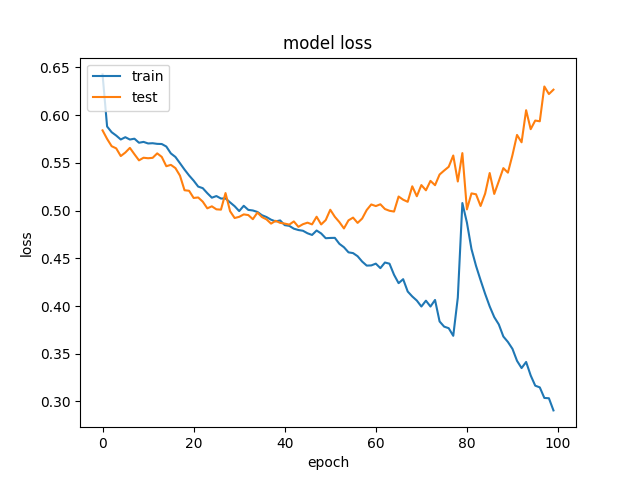
\includegraphics[width=3in]{loss.png}
\DeclareGraphicsExtensions.
\caption{Loss}
\label{fig_sim}
\end{figure}

\begin{figure}[h]
\centering
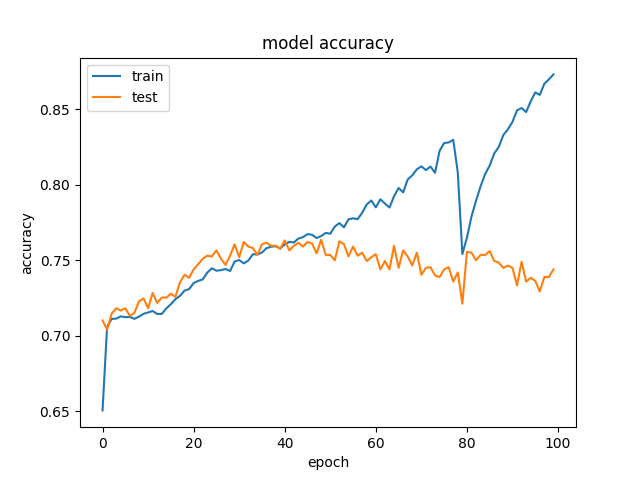
\includegraphics[width=3in]{accuracy.png}
\DeclareGraphicsExtensions.
\caption{Accuracy}
\label{fig_sim}
\end{figure}

\section{Conclusion}
From the preliminary experments, we were able to deduce that LSTM models are suitable to model DNA sequences effectively. Proceeding to the DNA classification, we developed an LSTM based architecture to classify given DNA sequences into plasmid or chromosomal. The architecture gives an accuracy of 0.89 which performs better than other models used for the same task, such as support vector machine and random forest classifier.

\section{Future interests}
There are several avenues of future interest to explore. First, we are actively exploring how to extend the model to process genetic variants in order to predict their functional consequences. Second, the model can be made fully recurrent so it can process sequences of arbitrary length, such as whole chromosome sequences, to generate sequential outputs.
In contrast, our current setup can only processes sequences of constant length with static outputs. A fully recurrent architecture may also benefit our effort to study variants since it would allow us to explore the long-range consequences of genetic variants.

\begin{thebibliography}{00}
\bibitem{} A deep learning approach to pattern
recognition for short DNA sequences, Akosua Busia, George E. Dahl, Clara Fannjiang, June 22 2018.

\bibitem{} Deep Recurrent Neural Network for Protein Function Prediction from Sequence, Xueliang Liu, Cornell University, 28 Jan 2017.

\bibitem{} DeepCpG: accurate prediction of single-cell
DNA methylation states using deep learning, Christof Angermueller, Heather J. Lee, Wolf Reik and Oliver Stegle, Genome Biology (2017)

\bibitem{} Improving protein disorder prediction by deep
bidirectional long short-term memory recurrent neural networks
Jack Hanson, Yuedong Yang, Kuldip Paliwal and Yaoqi Zhou, Oxford, October 26, 2016.

\bibitem{} Daniel Quang and Xiaohui Xie. Danq: a hybrid convolutional and recurrent deep neural network for quantifying the function of DNA sequences. bioRxiv, page 032821, 2015.

\bibitem{} Genotype-phenotype matching analysis of 38 Lactococcus lactisstrains using random forest methods,Jumamurat R Bayjanov, Marjo JC Starrenburg, Marijke R van der Sijde,
BMC Microbiology 2013.

\bibitem{} Qingda Zhou, Qingshan Jiang, Dan Wei, "A new method for classification in DNA sequence", Computer Science \& Education (ICCSE) 2011 6th International Conference on, pp. 218-221, 2011.

\bibitem{} A Brief Survey on Sequence Classification, Zhengzheng Xing, Jian Pei, Eamonn Keogh, ACM SIGKDD Explorations Newsletter, Volume 12 Issue 1, June 2010

\bibitem{} In Silico Detection and Typing of Plasmids,  Alessandra Carattoli, a Ea Zankari.

\bibitem{} Gene identification using a support vector machine for ORF classification, Lutz Krause, Alice C. McHardy  Tim W. Nattkemper.

\end{thebibliography}
\vspace{12pt}
\end{document}
